\section{Scelta dell'uscita}
Un'ambientazione realistica presenta tipicamente molteplici elementi, che contribuiscono ad aumentare la complessità della situazione da analizzare. \newline 
Ad esempio, pensando alla planimetria di un edificio, è inusuale che vi sia una sola uscita, in quanto una scelta del genere comporterebbe problemi sia dal punto di vista logistico sia da quello della sicurezza. \newline
Per determinare i probabili movimenti di una folla in uno scenario contraddistinto da più punti di interesse aventi lo stesso scopo, è necessario scegliere con cura la strategia da utilizzare per la combinazione delle varie forze in gioco, altrimenti si rischia di ottenere simulazioni poco attendibili.

\subsection{Descrizione della simulazione}
Lo scenario utilizzato è molto simile a quello impiegato nelle simulazioni del modello IMPACT: un ambiente limitato di dimensione quadrata con quattro uscite, al centro del quale è presente una zona di pericolo. Intorno ad essa, sono disposti casualmente 150 agenti cognitivi. \newline
In questo caso, non è possibile definire univocamente il movimento dei vari pedoni, in quanto, essendo presenti multiple uscite, non tutti hanno in comune lo stesso punto di arrivo. \newline
La stessa simulazione è stata ripetuta prima considerando come reazione responsabile del movimento il \texttt{BlendedSteering}, che utilizza la strategia basata sulla distanza, poi il \texttt{PrioritySteering}, che utilizza la strategia basata sulla massima vicinanza.

\subsection{Risultati ottenuti}
I momenti salienti in figura \ref{fig:multiple-exits-blended} dimostrano come l'utilizzo del \texttt{BlendedSteering} non sia adatto a descrivere la situazione e conduca a risultati inverosimili, dovuti al fatto che il pedone rimane perennemente indeciso su quale uscita scegliere in maniera particolare se si trova al centro della stanza, che è il luogo da cui dovrebbe avere più interesse a stare lontano. \newline
Ben diverso è il risultato nel caso si utilizzi il \texttt{PrioritySteering} (figura \ref{fig:multiple-exits-priority}), che determina un comportamento più simile a quello che si osserverebbe nella vita reale, contraddistinto da un iniziale allontanamento dal pericolo seguito dal raggiungimento dell'uscita più vicina.

\begin{figure}
    \centering
    \begin{subfigure}[b]{0.75\textwidth}
        \centering
        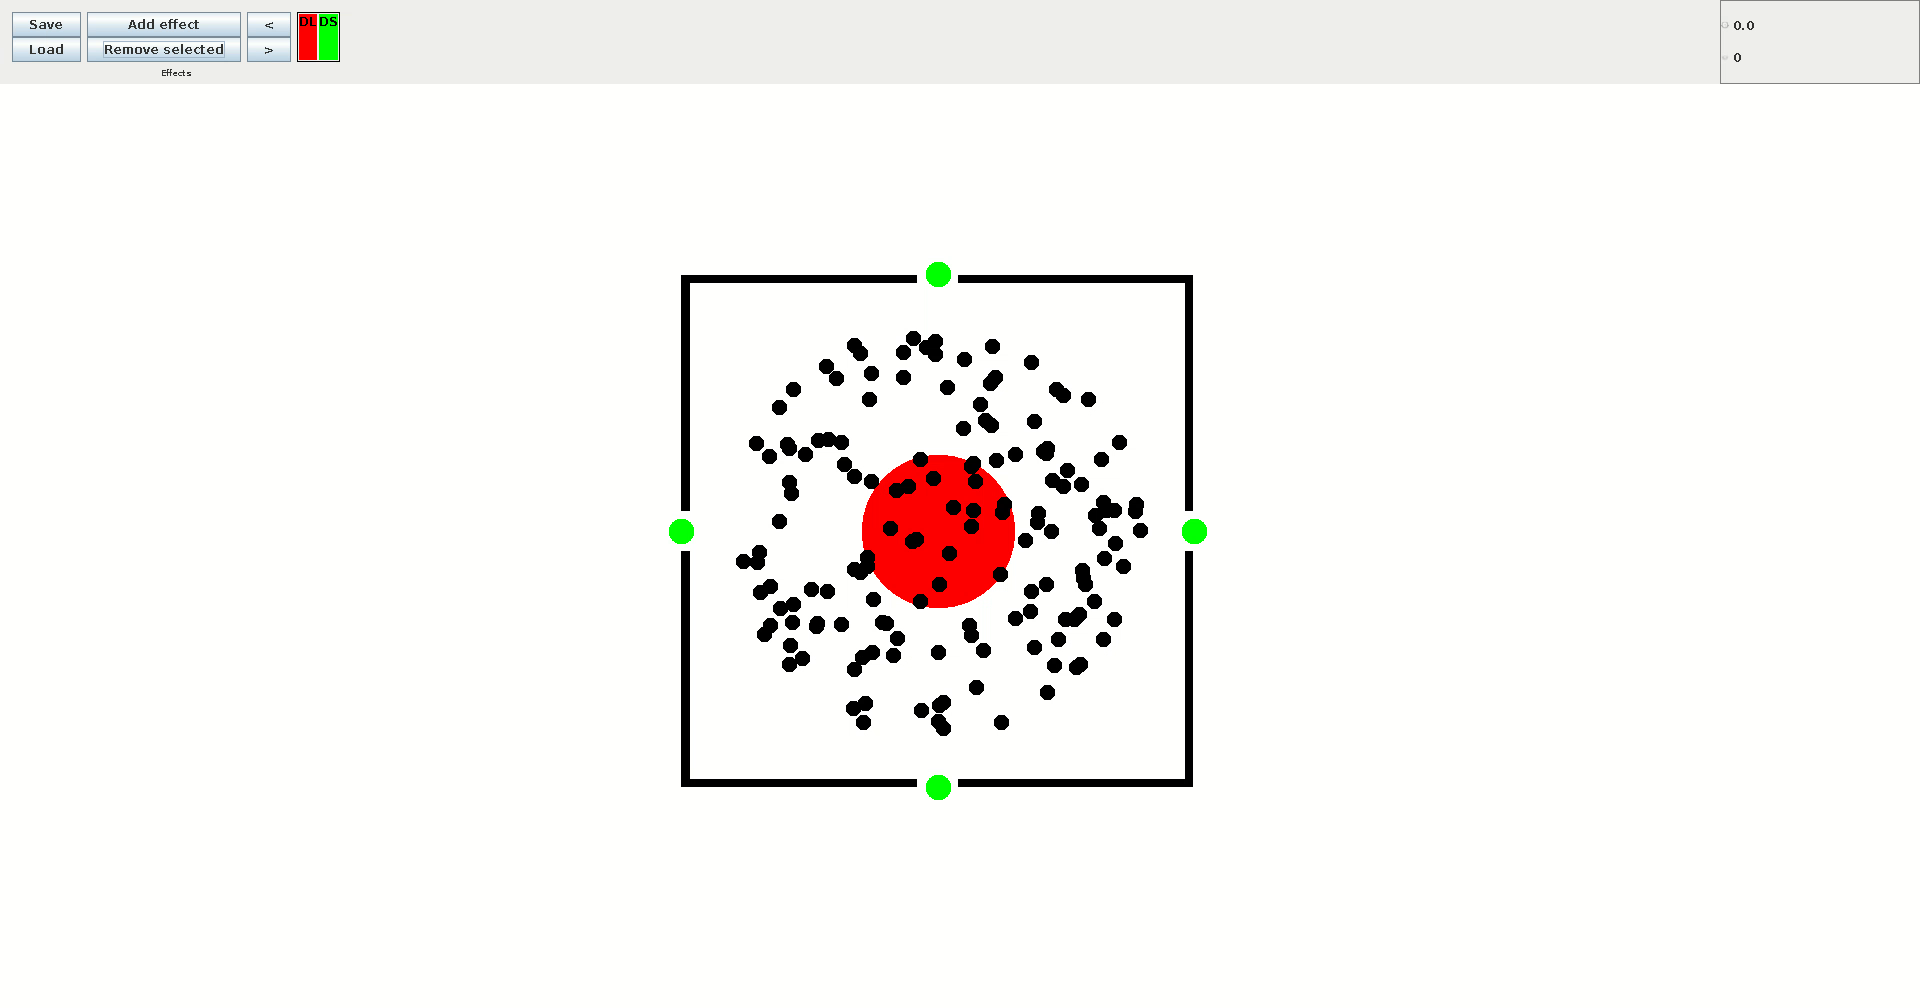
\includegraphics[width=\textwidth]{immagini/casi-studio/multiple-exits-blended-begin.png}
    \end{subfigure}
    \hfill
    \begin{subfigure}[b]{0.75\textwidth}
        \centering
        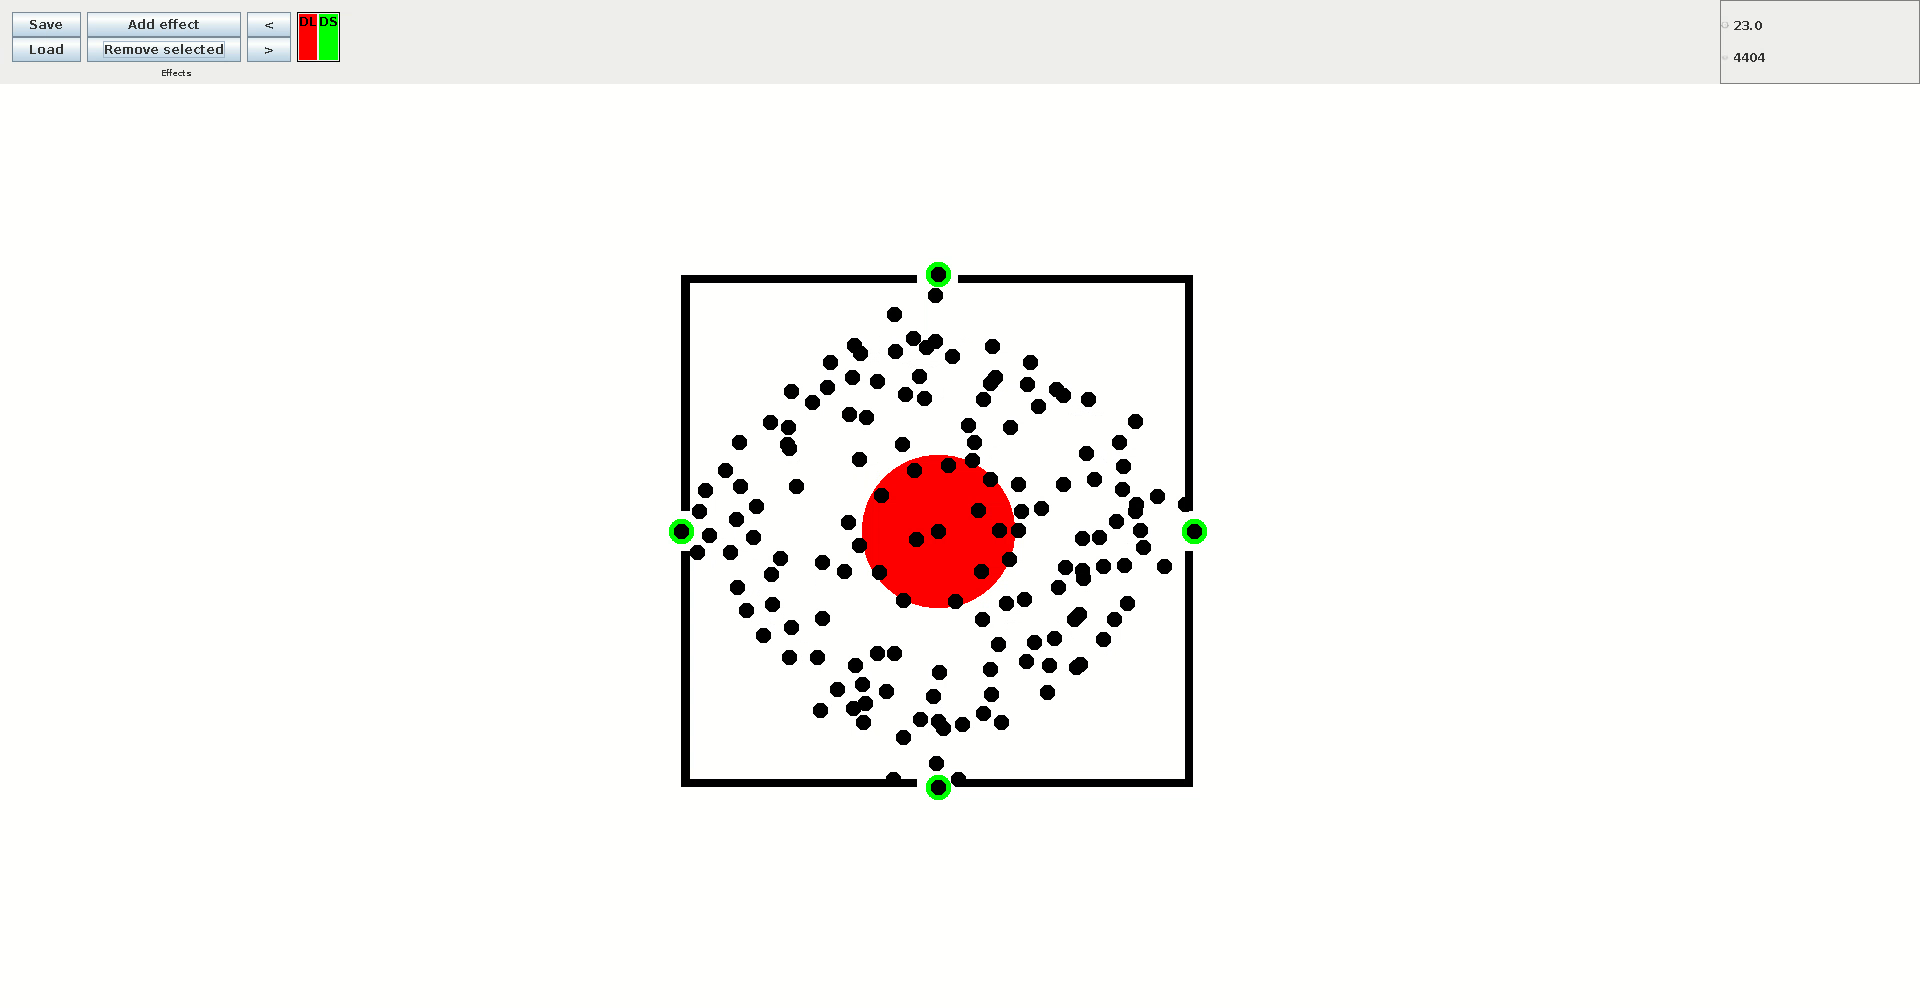
\includegraphics[width=\textwidth]{immagini/casi-studio/multiple-exits-blended-during.png}
    \end{subfigure}
    \hfill
    \begin{subfigure}[b]{0.75\textwidth}
        \centering
        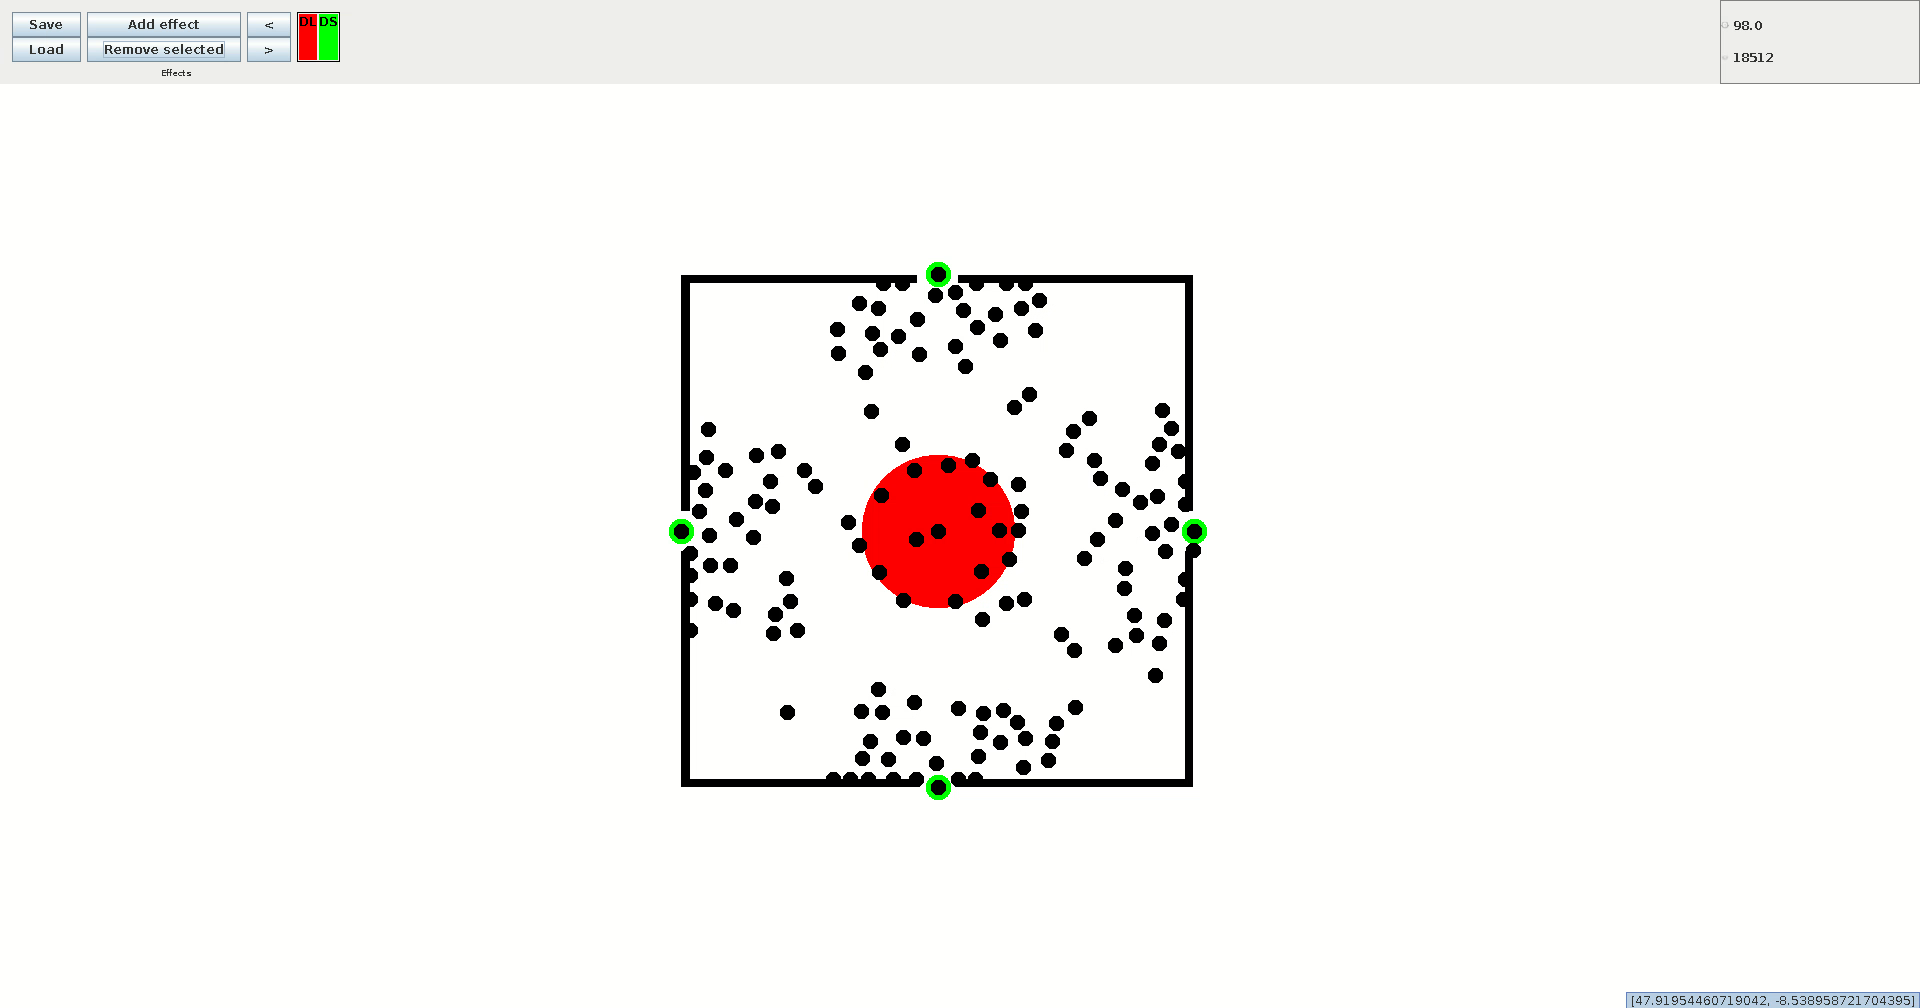
\includegraphics[width=\textwidth]{immagini/casi-studio/multiple-exits-blended-end.png}
    \end{subfigure}
    \caption{Fotogrammi salienti della simulazione sulla scelta dell'uscita utilizzando come strategia il \texttt{BlendedSteering}; le molteplici direzioni che il pedone è portato a seguire dai vari comportamenti di steering conducono a risultati inverosimili.}
    \label{fig:multiple-exits-blended}
\end{figure}

\begin{figure}
    \centering
    \begin{subfigure}[b]{0.75\textwidth}
        \centering
        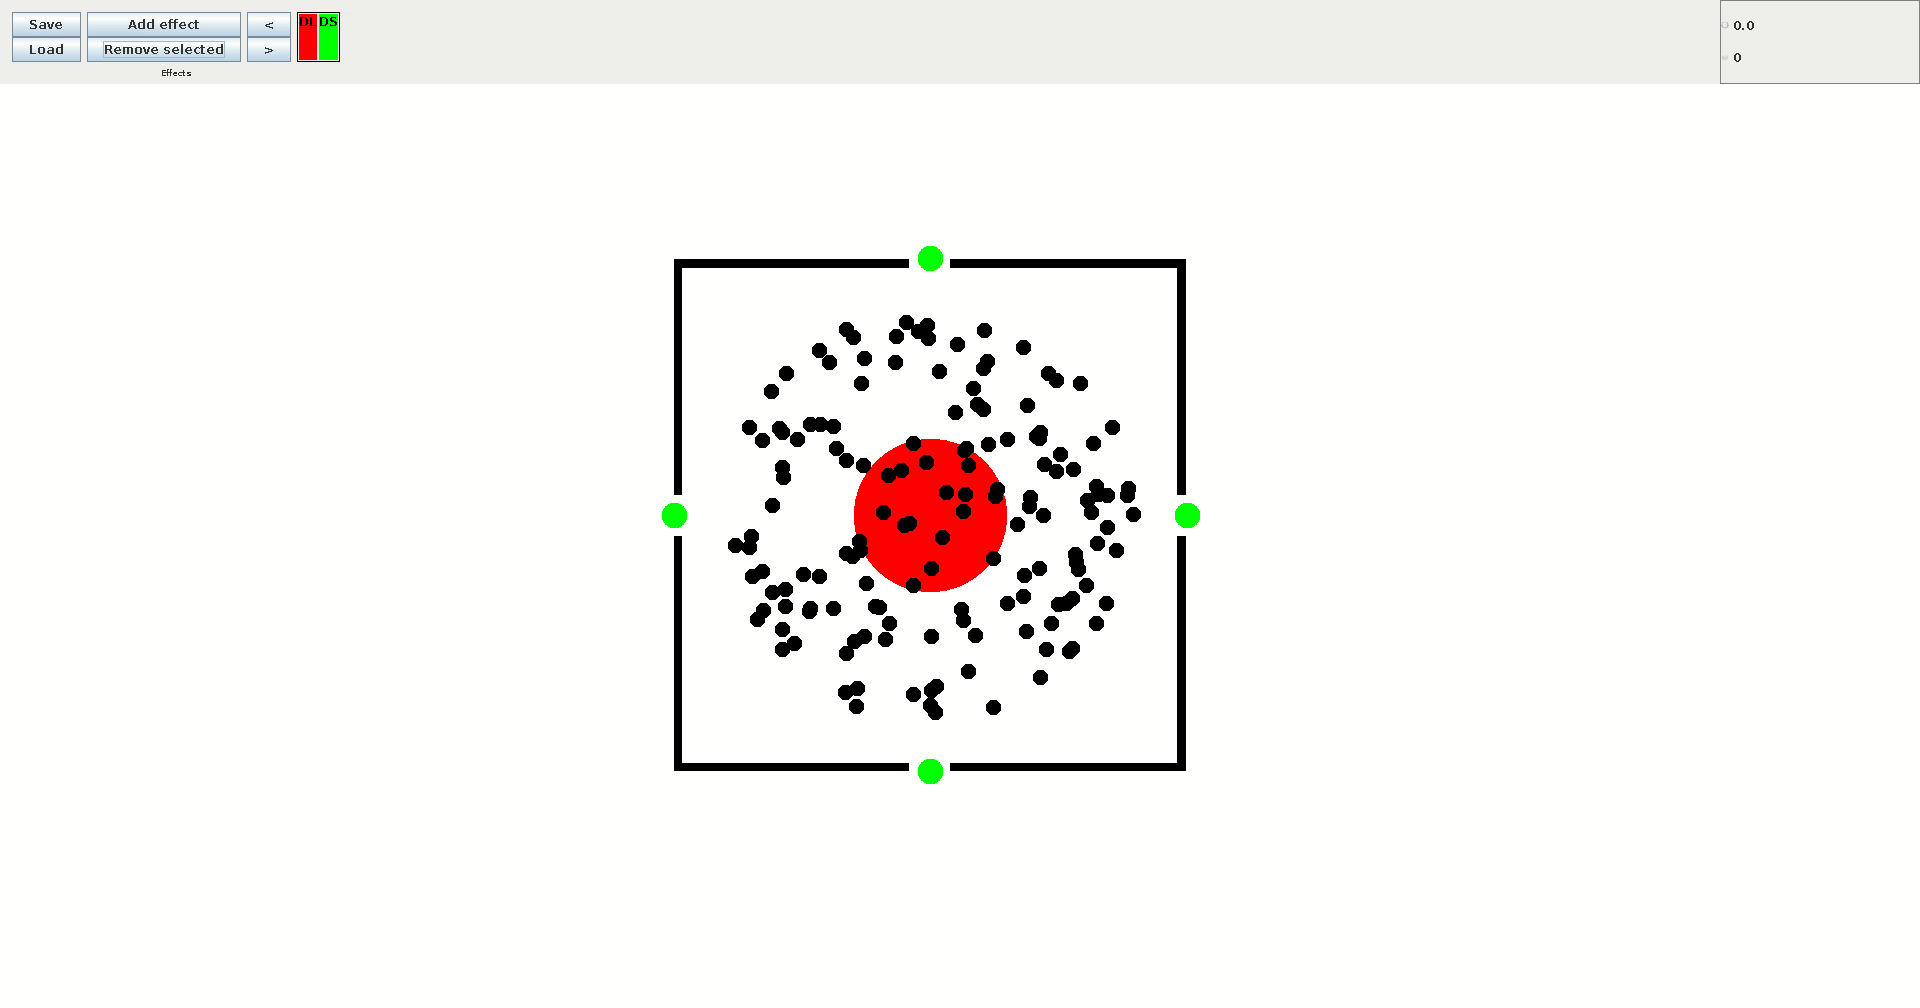
\includegraphics[width=\textwidth]{immagini/casi-studio/multiple-exits-priority-begin.png}
    \end{subfigure}
    \hfill
    \begin{subfigure}[b]{0.75\textwidth}
        \centering
        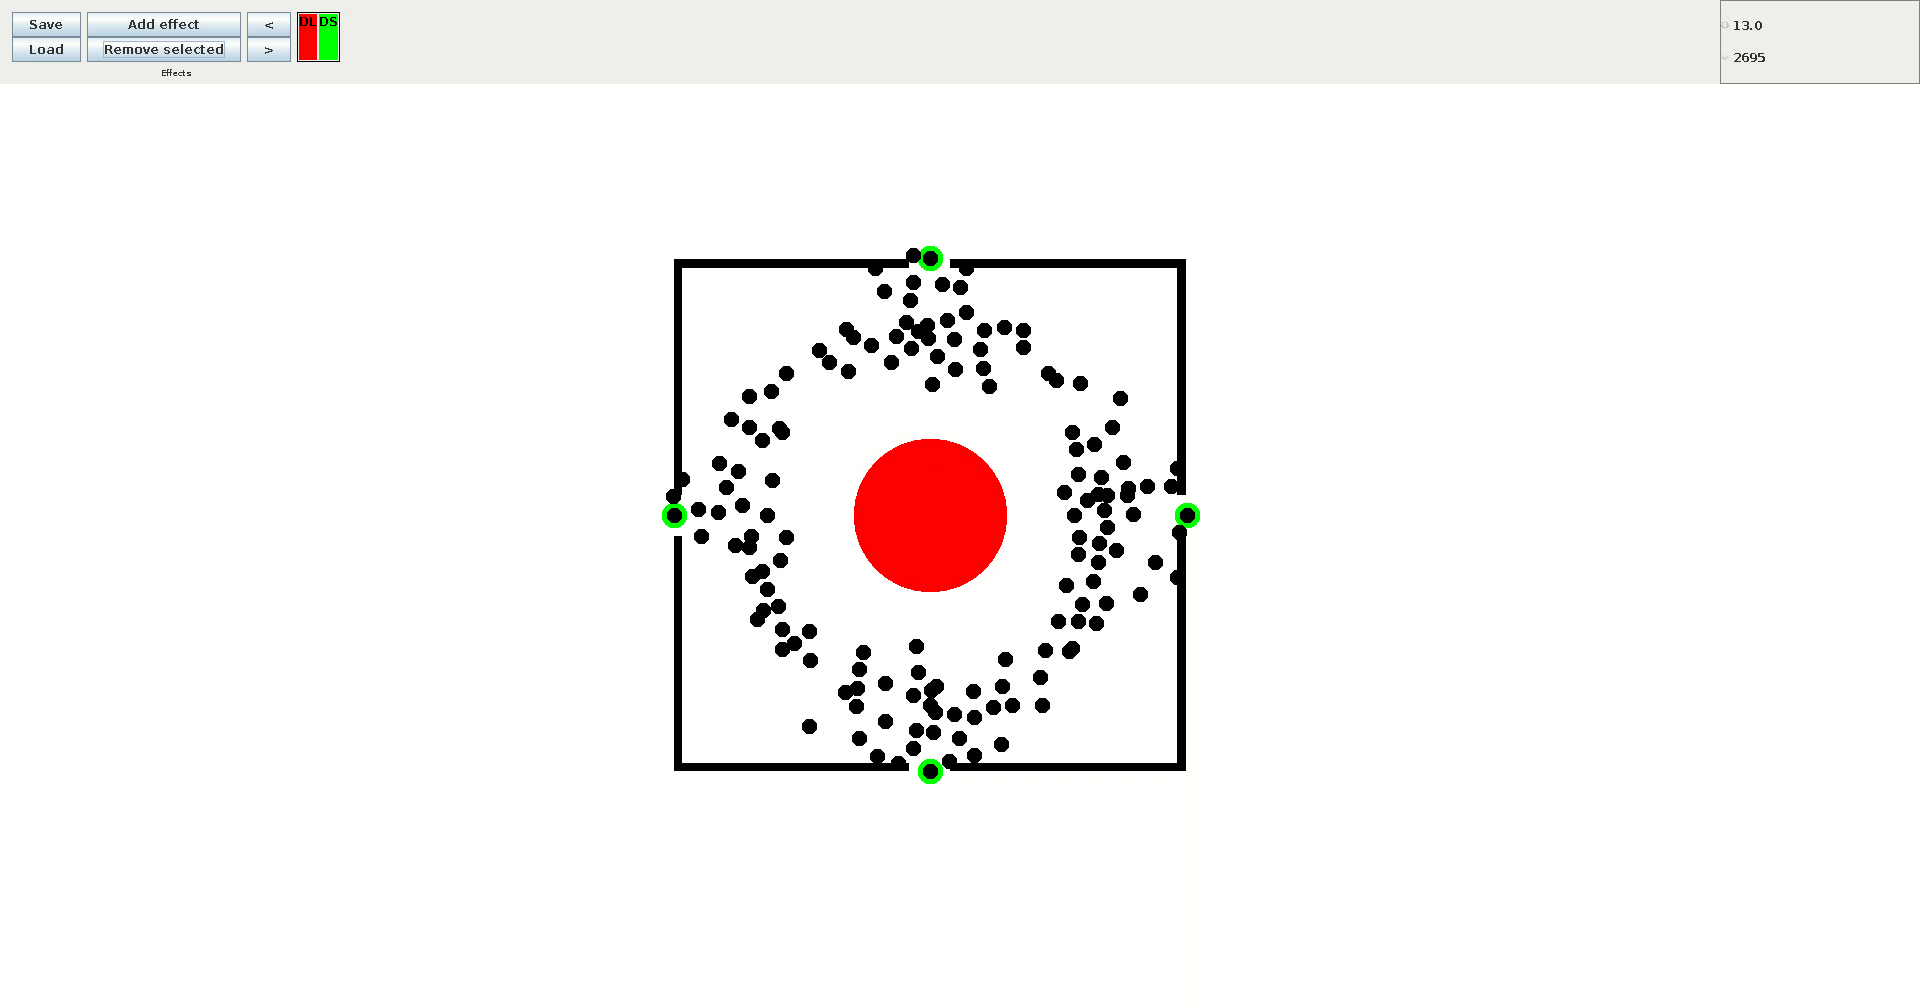
\includegraphics[width=\textwidth]{immagini/casi-studio/multiple-exits-priority-during.png}
    \end{subfigure}
    \hfill
    \begin{subfigure}[b]{0.75\textwidth}
        \centering
        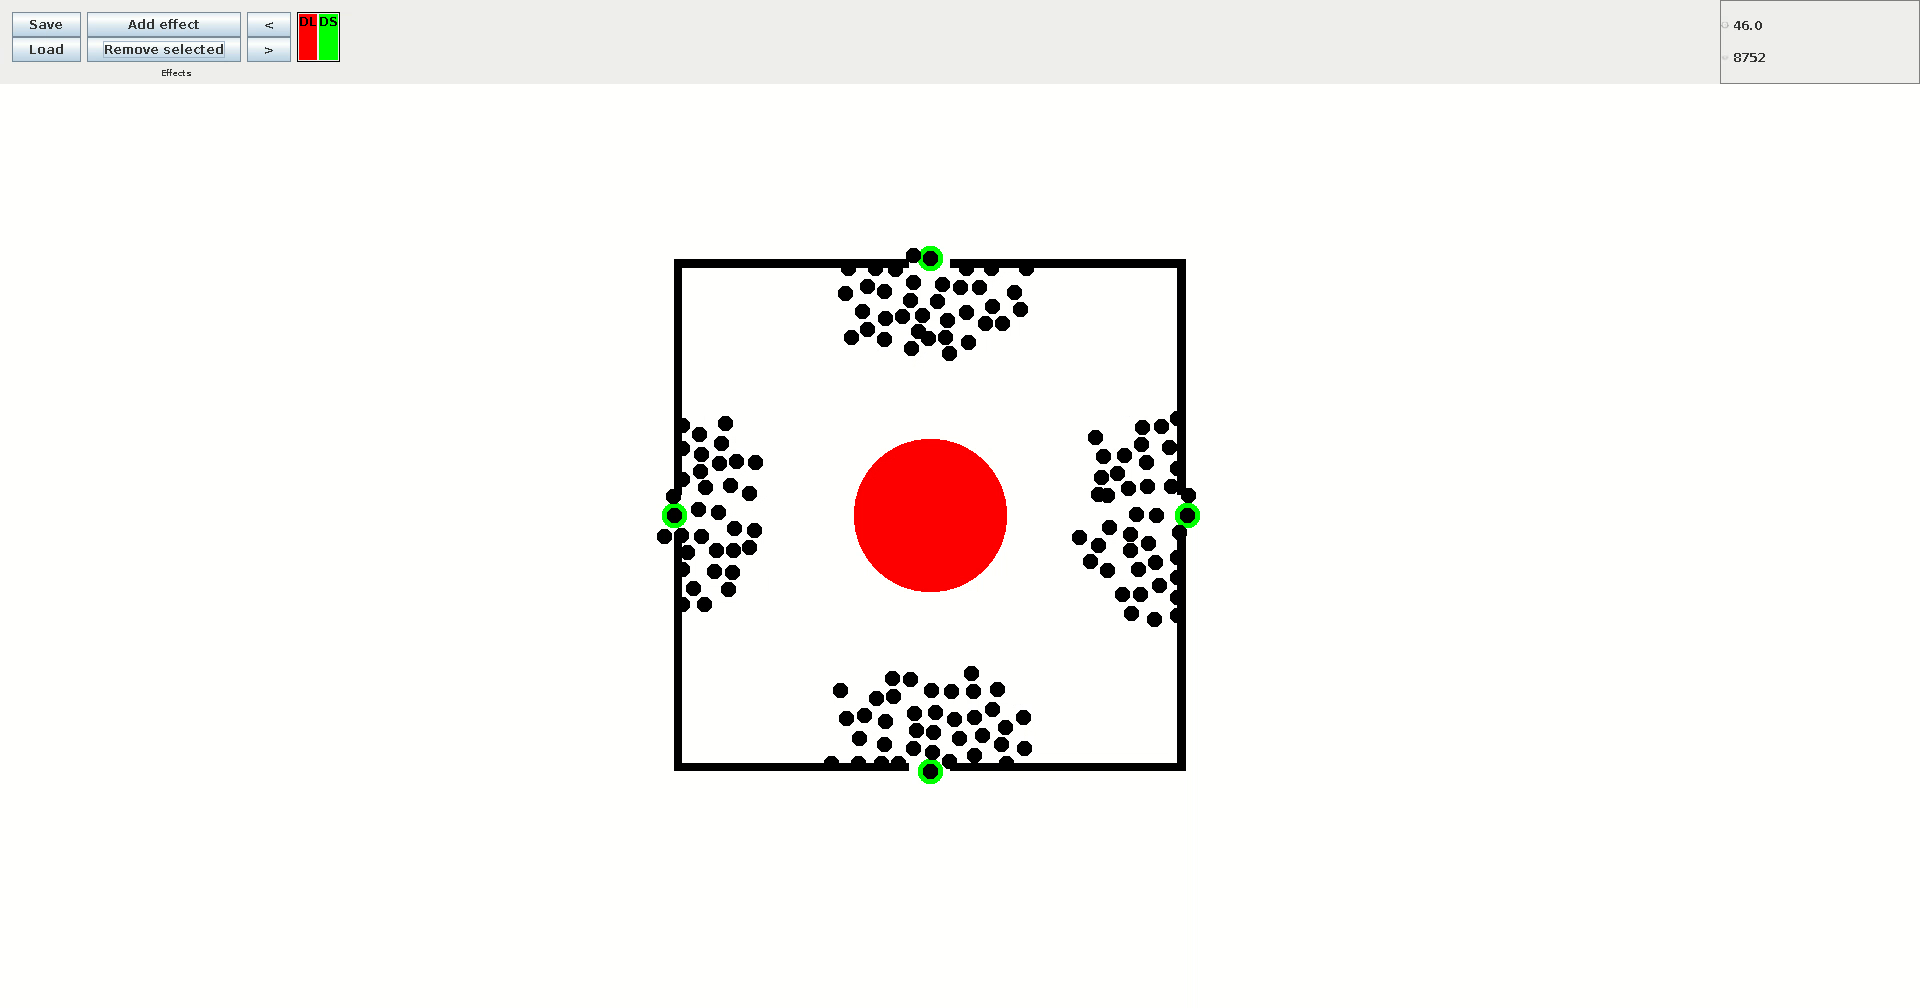
\includegraphics[width=\textwidth]{immagini/casi-studio/multiple-exits-priority-end.png}
    \end{subfigure}
    \caption{Fotogrammi salienti della simulazione sulla scelta dell'uscita utilizzando come strategia il \texttt{PrioritySteering}; definendo una priorità tra le azioni da eseguire, è possibile condurre i pedoni verso l'uscita loro più congeniale.}
    \label{fig:multiple-exits-priority}
\end{figure}